\section{Admission and terminal-coupling matching}
\label{sec:trajectories}

The exact map provides a stable class of densities. We now select trajectories
that stay in this class and reach a prescribed terminal kinetic coupling.
The coefficient calculation in Section~\ref{cal:section} is the input that
fixes their depth; terminal matching will then compare their full endpoint data.

\subsection{Initialization and admitted trajectories}
\label{rg:trajectories}

Here $j$ counts remaining layers: $b_N$ is the bare coupling and $b_0$
is terminal. The chronological free-history index is $h=N-j$, as in
the coefficient calibration and the introductory drift formula.

At free history zero, the unmasked quadratic energy is the
nearest-neighbor energy.  Its representation in the class has
all seven slots and all regular errors zero.  To construct the
covering gas, group the true bad bonds into connected
components after padding by a fixed multiple of
$R_*\log(100/t)$.  Assign every deleted mask row to a bad bond
witnessing its deletion, and retain that witness in the
component record.  The difference between the original energy
and the clipped energy is nonnegative.  Each bad bond supplies
at least $cb r_e^2\ge cp^2$ to this difference.  The remaining
deleted rows are nonnegative squares.  The weight of a
component is the exponential of minus its assigned difference,
with the indicators recording its exact bad-bond inventory.
These components have disjoint padded supports, or are joined
when their supports meet.  Their product therefore gives
exactly the original density.

Connected positioning and padding cost at most
$\exp(Cs\log M)$ for a record of load $s$.  The retained
$p^2$ reserve dominates this count and $e^{As}$ by
\eqref{rg:finite-choices}, proving the initial covering cap.
The initial weights are continuous in the precise bare coupling:
their geometric predicates use the fixed reference parameters
$H_j,t_j,\mathfrak m_j$, so only the exponential energy factors vary.
The retained reserve makes this continuity uniform in the covering
norm on each admitted coupling interval. For two nearby inputs with
the same free history, the comparison estimates
\eqref{rg:shape-comparison}--\eqref{rg:coupling-comparison} have
$\epsilon_h=0$ and preserve continuity of both the shape data and
the extracted coupling. Induction therefore gives a continuous
terminal-coupling map on every finite sequence of strictly admitted
inputs. This is the continuity used in the shooting argument below.

Write $\alpha_h,\kappa_h$ for the kicks on the canonical orbit
started from zero.  Theorem~\ref{thm:calibration}, proved in Section~\ref{cal:section}, gives
\begin{equation}
 \alpha_h=-\gamma+O_L(\rho_c^h),\qquad
 \kappa_h=-\frac{\gamma}{2\pi}+O_L(\rho_c^h),
 \qquad 0<\rho_c<1 .
 \label{rg:calibrated-kicks}
\end{equation}
The regular error $\Delta$ is not used in that formal
calculation.  It is bounded for the actual trajectory by
Theorem~\ref{thm:rg-closure}.

\begin{proposition}[Admission and shooting]
\label{rg:admission}
Fix $L,P_0,H$ as above, increasing $H$ if necessary, and put
$I_H=[.9H,1.1H]$.  Every sufficiently large prescribed bare
coupling $b$ has a depth $N$ for which the nearest-neighbor
trajectory remains in all its admitted bands and ends at a
coupling in $I_H$.  Conversely, for every $N\ge1$ and every
$h_0\in I_H$ there is a bare coupling $b_N(h_0)$ whose admitted
trajectory of depth $N$ ends exactly at $h_0$.

For each of these trajectories, uniformly in its depth and
terminal value,
\begin{equation}
 N\log L=\pi b-\tfrac12\log b+O_{L,H}(1),
 \qquad
 L^N\asymp_{L,H} b^{-1/2}e^{\pi b}.
 \label{rg:scale-calibration}
\end{equation}
No uniqueness of the shooting value is asserted or needed.
\end{proposition}
\begin{proof}
Set $c_{\log}=1/(2\pi)$ and define
\[
 \vartheta_j=H_j+c_{\log}\log(H_j/H).
\]
It obeys
\[
 \vartheta_j-\vartheta_{j-1}
    =\gamma+\frac{\gamma}{2\pi H_j}
                       +O_L(H_j^{-2}).
\]
Choose $N$ so that $|b-\vartheta_N|\le C_L$, and run the exact
map only until its first possible exit.  Put
$D_j=b_j-\vartheta_j$.  Sum
\eqref{rg:coupling-step} and \eqref{rg:calibrated-kicks} along
an admitted initial segment.  The exponential kick errors
have bounded total sum, as does $\sum_jH_j^{-1.05}$ at fixed
$L,H$.  The denominator difference is bounded by
\[
 |b_j^{-1}-H_j^{-1}|
 \le C\{\log(2+H_j/H)+|D_j|\}/H_j^2 .
\]
Consequently, including a first candidate output position,
\begin{equation}
 |D_j|\le C_L+
 C_L\sum_{r=j+1}^N
       \frac{\log(2+H_r/H)+|D_r|}{H_r^2}.
 \label{rg:first-exit-bound}
\end{equation}
The constant can be chosen bounded as $H$ is increased.
Both coefficient sums on the right are $O_L(H^{-1})$.
Taking a maximum and then increasing $H$ gives
$|D_j|\le2C_L$ on this entire segment.
Also $\sup_{x\ge H}\log(x/H)/x=1/(eH)$.
Thus $\vartheta_j+[-2C_L,2C_L]$ lies strictly inside
$[H_j/2,2H_j]$ for every $j$, and its value at $j=0$
lies in $I_H$.  A first exit is impossible.  This proves
the assertion for prescribed $b$.

For exact shooting, vary the initial value in
$[.6H_N,1.4H_N]$.  On every admitted segment from layer
$k$ to layer $j<k$, the same equations, using only
$b_r\ge H_r/2$, give
\begin{equation}
 |(b_j-H_j)-(b_k-H_k)|
       \le C_L+C_L(k-j)/H .
 \label{rg:barrier-bound}
\end{equation}
Call a value high if a strictly admitted initial segment
reaches $b_k>1.25H_k$, or if its strictly admitted full run
ends above $h_0$.  Define low with $b_k<.75H_k$ or a terminal
value below $h_0$.  These classes are open by continuity.
They are nonempty because they contain respectively the
upper and lower endpoints of the initial interval.

They are disjoint.  Indeed an upper mark and a lower mark
would make the left side of \eqref{rg:barrier-bound} at least
$(H_j+H_k)/4$, while its right side is
$C_L+C_L(k-j)/H$.  For large $H$, the former exceeds the
latter, since $H_k-H_j=\gamma(k-j)$.  An upper mark and a
terminal value at most $h_0$ instead give a lower bound
$H_k/4-.1H$; the same comparison rules this out.
The argument with lower marks is identical.

A connected interval cannot be the union of two nonempty
disjoint open subsets.  An initial value outside both
classes cannot leave an admitted band: every step changes
the coupling by at most $C_L$, and $H$ is large enough that
a first exit must have been preceded by one of the strict
internal marks.  It therefore reaches layer zero, and its
terminal value is neither above nor below $h_0$.  This is
the required shot.

For a shot, $D_0=h_0-H=O(H)$.  Sum the same difference equation
backwards from layer zero.  The sums of the inhomogeneous
errors are bounded and $\sum_rH_r^{-2}=O_L(H^{-1})$.
Taking the maximum on any finite run absorbs its coefficient
and yields $D_j=O_{L,H}(1)$ uniformly in $j,N$.  For either
construction,
\[
 b=H+\gamma N+\frac1{2\pi}\log((H+\gamma N)/H)
                                      +O_{L,H}(1).
\]
The difference between $\log(H+\gamma N)$ and $\log b$
is bounded, and tends to zero as $N$ grows.  Multiplying by
$\pi$ gives \eqref{rg:scale-calibration}.
\end{proof}

\subsection{Matching at a common terminal coupling}
\label{rg:terminal}

Figure~\ref{fig:matched-trajectories} displays the two boundary conditions
used in the following comparison.
\begin{figure}[tbp]
  \centering
  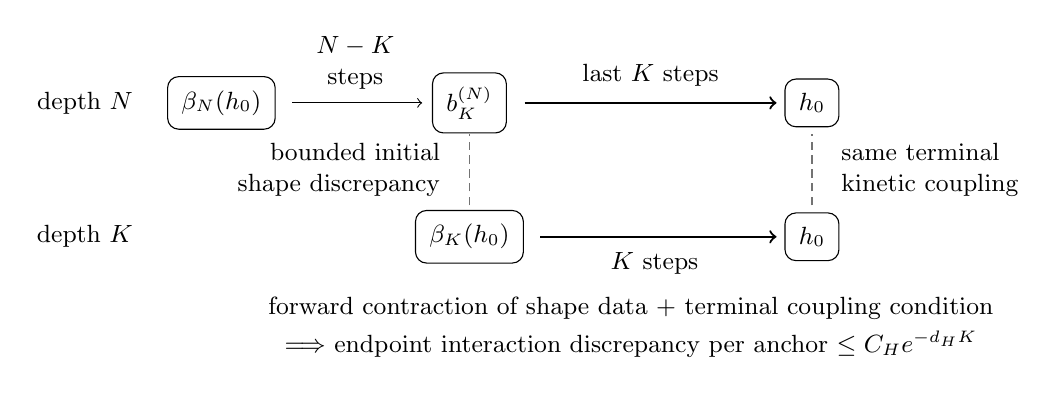
\begin{tikzpicture}[x=1cm,y=1cm,font=\small]
    \node[anchor=east] at (0,1.7) {depth $N$};
    \node[draw,rounded corners,inner sep=5pt] at (1.0,1.7)
      {$\beta_N(h_0)$};
    \draw[->] (1.9,1.7) -- (3.55,1.7);
    \node[above,align=center] at (2.7,1.75) {$N-K$\\steps};
    \node[draw,rounded corners,inner sep=5pt] at (4.15,1.7)
      {$b_K^{(N)}$};
    \draw[->,thick] (4.85,1.7) -- (8.05,1.7);
    \node[above] at (6.45,1.78) {last $K$ steps};
    \node[draw,rounded corners,inner sep=5pt] at (8.5,1.7) {$h_0$};

    \node[anchor=east] at (0,0) {depth $K$};
    \node[draw,rounded corners,inner sep=5pt] at (4.15,0)
      {$\beta_K(h_0)$};
    \draw[->,thick] (5.05,0) -- (8.05,0);
    \node[below] at (6.5,-0.08) {$K$ steps};
    \node[draw,rounded corners,inner sep=5pt] at (8.5,0) {$h_0$};

    \draw[densely dashed,black!55] (4.15,0.4) -- (4.15,1.3);
    \node[anchor=east,align=right] at (3.9,0.85)
      {bounded initial\\shape discrepancy};
    \draw[densely dashed,black!55] (8.5,0.4) -- (8.5,1.3);
    \node[anchor=west,align=left] at (8.75,0.85)
      {same terminal\\kinetic coupling};

    \node[align=center] at (6.2,-1.15)
      {forward contraction of shape data + terminal coupling condition\\[3pt]
       $\Longrightarrow$ endpoint interaction discrepancy per anchor $\le C_H e^{-d_H K}$};
  \end{tikzpicture}\par\medskip
  \caption{The comparison aligns the last $K$ blocking steps of two
  admitted trajectories with $N\ge K$. Here $b_K^{(N)}$ is the longer
  trajectory's coupling after its first $N-K$ steps. Their kinetic couplings agree
  at the terminal scale. Their complete endpoint laws need not agree:
  contraction bounds the discrepancy in their local interaction data,
  while bulk scalars are tracked separately. The bound is uniform in
  the number $N-K$ of earlier steps.}
  \label{fig:matched-trajectories}
\end{figure}

\FloatBarrier

\begin{theorem}[Matched endpoint densities]
\label{rg:matching}\label{thm:matched-endpoint}
Let $N\ge K\ge1$, and choose any two admitted nearest-neighbor
trajectories of these depths with the same terminal coupling
$h_0\in I_H$.  On every common admitted terminal period $m$,
write their exact endpoint densities as
\[
 \rho_r(V)=e^{v_rm^2}e^{X_r(V)}\Xi_r(V),\qquad r=N,K,
\]
using common compatible label lists.  The numbers $v_r$ are
independent of $m$.  There are constants $C_H,d_H>0$,
independent of $N,K,h_0,m$, such that
\begin{align}
 \|X_N-X_K\|_\infty
       &\le C_Hm^2e^{-d_HK},\nonumber\\
 \sup_x\sum_{\ell:x\in P_\ell}
      e^{As_\ell}\|k_{N,\ell}-k_{K,\ell}\|_\infty
       &\le C_He^{-d_HK}.
 \label{rg:terminal-difference}
\end{align}
All the endpoint class bounds hold uniformly.  In particular,
with $t=t_0$, the canonical part of $-X_r$ is bounded by
$C_Lm^2(Ht^4+t^2)$ and its error part by $m^2H^{-2.05}$.
Every covering support has a connected hull of at most
$R_Hs_\ell$ sites.  Changing a set $B$ of endpoint spins
changes $X_r$ by at most $D_H|B|$.  The constants $R_H,D_H$
can be chosen polynomial in $H$.
\end{theorem}
\begin{proof}
Compare the last $K$ layers, indexed by $j=K,\ldots,0$.
At their common upper layer both shape data are within the
fixed caps, so $u_K\le C$.  Their free histories differ;
the shallower one at layer $j$ is $K-j$, giving
$\epsilon_j\le L^{-(K-j)}$.  Their couplings agree at the
opposite end: $\lambda_0=0$.

Set $\eta=C_LH^{-b_*}$, enlarging its constant if necessary,
and $f_j=C_LH_j^CL^{-(K-j)}$.  The step inequalities imply
\[
 u_{j-1}\le q u_j+\eta|\lambda_j|+f_j,\qquad
 |\lambda_j|\le
 a|\lambda_{j-1}|+aC_Lu_j+af_j,\quad
 a=(1-\eta)^{-1}.
\]
Choose $\rho$ with $\max(q,L^{-1})<\rho<1$, and then
increase $H$ until $a\rho<1$.  Put
$w_j=\rho^{K-j}$,
$U=\max_{0\le j\le K}u_j/w_j$, and
$W=\max_{0\le j\le K}|\lambda_j|/w_j$.
For $F_K=C_{L,H}(1+K)^C$ we have $f_j\le F_Kw_j$.
Iterating the first inequality from $K$ and the second
from $0$ gives
\[
 U\le u_K+\frac{\eta W+F_K}{\rho-q},\qquad
 W\le\frac{a(C_LU+F_K)}{1-a\rho}.
\]
Choose $H$ so that the product of the two coefficients
linking $U$ and $W$ is less than $1/2$.
It follows that
\begin{equation}
 u_j+|\lambda_j|
       \le C_{L,H}(1+K)^C\rho^{K-j}.
 \label{rg:two-end-bound}
\end{equation}
This argument requires neither a bound on the ratio of
the two bare couplings nor uniqueness of either shot.

At $j=0$ the shape estimate and the free-history error
$O(L^{-K})$ give the covering estimate in
\eqref{rg:terminal-difference}.  They also bound the
regular negative-log difference per anchor, including
the difference of the clipped kinetic kernels; their
displayed couplings are equal.  Summing over $m^2$ anchors
gives the first estimate.  A fixed polynomial in $K$
is absorbed by decreasing the positive exponential rate.
Uniformity in $h_0$ follows from its compact admitted
interval and the same constants in the step estimates.

At each step only a bulk scalar was extracted.  The number
of sites at layer $j$ is $m^2L^{2j}$, so the sum of all
extracted scalars is exactly $v_rm^2$ with $v_r$ independent
of $m$.  All period discrepancies were kept in the winding
lists.

The remaining statements follow directly from the class
norms at $j=0$.  On a canonical graph,
$|y_o(x)|\le Ct$ times its path length; the exponential
coefficient norm sums the resulting fixed powers, giving
$C_L(Ht^4+t^2)$ per anchor.  The error bound is its cap.
The complete record gives a hull of $O(\mathfrak m_0^2s_\ell)$ sites.
For a local change of spins, sum only terms whose complete
support meets the changed set, charging each term to one
such site.  Conversion from anchored to support-hit sums
costs fixed position moments, and all test neighborhoods
have polynomial size in $H$.  The kinetic terms and their
mask tests obey the same bound by the free exponential
moments.  This gives $D_H$ polynomial in $H$.
\end{proof}

The endpoint densities in this theorem are strictly positive:
they are repeated integrals of the positive microscopic
density against the strictly positive kernel
\eqref{rg:observation}.  More quantitatively, changing $B$
endpoint spins changes the logarithm of the true endpoint
density by at most $C_LH|B|$.  For each fixed input the
last observation densities have this ratio bound, since
their coupling is in a fixed band of order $H$ and chord
lengths on $S^3$ are bounded.  Integrating their ratio
inequality against the positive preceding-layer measure
preserves it.  This positivity statement concerns the
complete density; the individual covering weights remain
allowed to have either sign.


